%%% LaTeX Template: Two column article
%%%
%%% Source: http://www.howtotex.com/
%%% Feel free to distribute this template, but please keep to referal to http://www.howtotex.com/ here.
%%% Date: February 2011

%%% Preamble
\documentclass[landscape,	DIV=calc,%
							paper=letter,%
							fontsize=10pt,%
							twocolumn]{scrartcl}	 					% KOMA-article class

\makeatletter
\newcommand\notsotiny{\@setfontsize\notsotiny{6.5}{7.5}}
\makeatother
\usepackage{lipsum}													% Package to create dummy text

\usepackage[margin=.6in,footskip=0.25in]{geometry}

\usepackage[english]{babel}										% English language/hyphenation
\usepackage[protrusion=true,expansion=true]{microtype}				% Better typography
\usepackage{amsmath,amsfonts,amsthm}					% Math packages
\usepackage[pdftex]{graphicx}									% Enable pdflatex
\usepackage[svgnames]{xcolor}		

\usepackage{sourcecodepro}
\usepackage[T1]{fontenc} 

\usepackage{listings} 

\definecolor{codegreen}{rgb}{0,0.9,0}
\definecolor{codegray}{rgb}{0.55,0.55,0.55}
\definecolor{codepurple}{rgb}{0.58,0,0.82}
\definecolor{backcolour}{rgb}{0.95,0.95,0.92}

\definecolor{commentgreen}{RGB}{2,112,10}
\definecolor{eminence}{RGB}{108,48,130}
\definecolor{weborange}{RGB}{255,165,0}
\definecolor{frenchplum}{RGB}{129,20,83}
\definecolor{CustomDarkRed}{RGB}{175, 0, 0} 
 

\lstdefinestyle{mystyle}{
    language=python,
    %backgroundcolor=\color{codegray},   
    commentstyle=\color{codegray},
    keywordstyle=\bfseries\color{CustomDarkRed},
    numberstyle=\tiny\color{codegray},
    stringstyle=\color{blue},
    basicstyle=\ttfamily\notsotiny,
    breakatwhitespace=false,         
    breaklines=true,                 
    captionpos=b,                    
    keepspaces=true,                 
    numbers=left,                    
    numbersep=5pt,                  
    showspaces=false,                
    showstringspaces=false,
    showtabs=true,                  
    tabsize=2,
    frame=tb, 
}

\lstset{style=mystyle}
% Enabling colors by their 'svgnames'
\usepackage[hang, small,labelfont=bf,up,textfont=it,up]{caption}	% Custom captions under/above floats
\usepackage{epstopdf}												% Converts .eps to .pdf
\usepackage{subfig}													% Subfigures
\usepackage{booktabs}												% Nicer tables
\usepackage{fix-cm}													% Custom fontsizes



%%% Custom sectioning (sectsty package)
\usepackage{sectsty}													% Custom sectioning (see below)
\allsectionsfont{%															% Change font of al section commands
	\usefont{OT1}{phv}{b}{n}%										% bch-b-n: CharterBT-Bold font
	}

\sectionfont{%																% Change font of \section command
	\usefont{OT1}{phv}{b}{n}%										% bch-b-n: CharterBT-Bold font
	}



%%% Headers and footers
\usepackage{fancyhdr}												% Needed to define custom headers/footers
	\pagestyle{fancy}														% Enabling the custom headers/footers
\usepackage{lastpage}	

% Header (empty)
\lhead{}
\chead{}
\rhead{}
% Footer (you may change this to your own needs)
\lfoot{\footnotesize \texttt{HowToTeX.com} \textbullet ~Two column article template}
\cfoot{}
\rfoot{\footnotesize page \thepage\ of \pageref{LastPage}}	% "Page 1 of 2"
\renewcommand{\headrulewidth}{0.0pt}
\renewcommand{\footrulewidth}{0.4pt}



%%% Creating an initial of the very first character of the content
\usepackage{lettrine}
\newcommand{\initial}[1]{%
     \lettrine[lines=3,lhang=0.3,nindent=0em]{
     				\color{DarkGoldenrod}
     				{\textsf{#1}}}{}}



%%% Title, author and date metadata
\usepackage{titling}															% For custom titles

\newcommand{\HorRule}{\color{DarkGoldenrod}%			% Creating a horizontal rule
									  	\rule{\linewidth}{1pt}%
										}
%%begin novalidate
\pretitle{\vspace{-70pt} \begin{flushleft} \HorRule 
				\fontsize{50}{50} \usefont{OT1}{phv}{b}{n} \color{DarkRed} \selectfont 
				}
    \usepackage[hidelinks]{hyperref}
\title{Easier Analytics }					% Title of your article goes here
\posttitle{\\\vspace{3mm}
\Large Simpler, smarter, faster, more
flexible and understandable
\par\end{flushleft}\vskip 0.5em}

\preauthor{\begin{flushleft}
					\large \lineskip 0.5em \usefont{OT1}{phv}{b}{sl} \color{DarkRed}}
     
\author{Tim Menzies and the EZ gang }											% Author name goes here
\postauthor{\footnotesize \usefont{OT1}{phv}{m}{sl} \color{Black} 
					North CarolinA State University	\\~\\
      Package: \url{https://pypi.org/project/ezr/0.1.0/}\\
      Source: \url{http://github.com/timm/ezr}\\
     Latex: \url{http://github.com/timm/ezr-tex}\\
     {\textcopyright} 2024 by Tim Menzies and the EZ gang is licensed under \textcolor{DarkRed}{Creative Commons Attribution-ShareAlike 4.0 International}
    \LARGE ~\ccLogo  
~\ccAttribution  
~\ccShareAlike  \par\end{flushleft}\vspace{-4mm}\HorRule}
%%end novalidate
\date{}	
\usepackage{ccicons}% No date
\usepackage{enumitem}
\setlist[itemize]{noitemsep}


%%% Begin document
\begin{document}
\maketitle
\thispagestyle{fancy} 			% Enabling the custom headers/footers for the first page 
% The first character should be within \initial{}
\initial{W}\textbf{e show
how to simplify the process of analytics, which
involves extracting high-quality  insights from large quantities
of data. We advocate for more efficient and  accessible analytical
methods that require fewer data samples and less  complexity. This
allows for easier verification and understanding of results. We
highlights the benefits of using incremental methods  in building
models that can provide valuable insights with minimal data.~\\~\\ 
This  work can be viewed as a (polite) protest
against  the prevailing preference for complex solutions
in the industry,  suggesting that simplicity could offer more
practical and appreciable benefits but is often overlooked due to
commercial interests. The call is for a shift towards simplicity
in analytics, making it faster, smarter, and more flexible, to
better serve practical needs and enhance comprehensibility.}


\section*{Introduction}

Suppose we want to use data to make policies-- about what to do,
what to avoid, what to do better, etc etc. How to do that?

This process is called {\em analytics}, i.e. the reduction of large
amounts of low-quality data into tiny high-quality statements. Think of it like
``finding the diamonds in the dust``.

Many people have been doing data-driven analytics for decades.  So
it seems the right time  to ask how can we make  analytics  simpler,
smarter, faster, more flexible and more understandable?

For example,  according to Tom Zimmermann (from Microsoft Research),
there are many things we want to do with analytics:

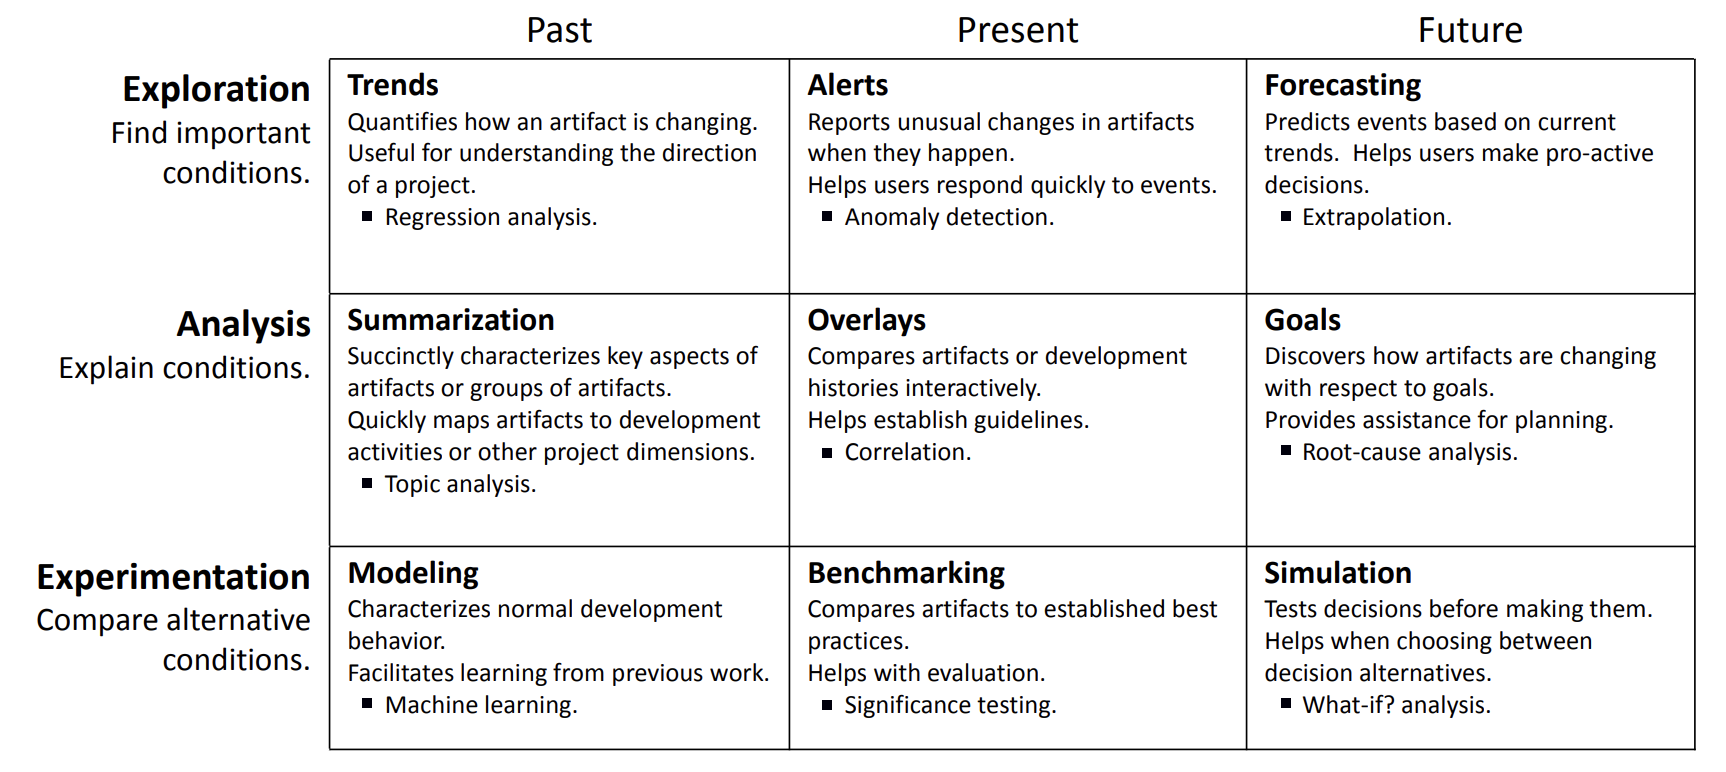
\includegraphics[width=\linewidth]{Buse.png} 

Note all the different algorithms in all the boxes.  Before we knew
better:
\begin{itemize}
    \item 
 We used to study those algorithms as separate  things. Now we see
them as very similar things, all of which call the same underling
structure. This means that  once we code one of them, we can quickly 
code up the rest. 
\item We 'd explore 100,000s of possibilities to find patterns in
the data (e.g. during a "what-if" query).  But these days, I can
do the same analysis with 30 samples, or 
less\footnote{Using semi-supervised multi-objective optimization via
sequential model optimization (which is all described, later in
this document).} 
This means
if someone wants to check my conclusions, they only need to review
a few dozen samples.  Such a review was impossible using prior
methods since the reasoning was so complicated.


Why can I do things so easily? Well,  based on three decades of work
on analytics [^pigs] (which includes the work of 20 Ph.D. students,
hundreds of research papers and millions of dollars in research
funding) I say:

- When building models, there are incremental methods that can find
models after very few samples.
- This is because the main message of most models is contained in
just a few variables [:keys].

[^keys]: Menzies, Tim, David Owen, and Julian Richardson. "The
strangest thing about software." Computer 40.1 (2007): 54-60
https://ieeexplore.ieee.org/stamp/stamp.jsp?arnumber=4069195

I'm not the first to say these things [^semi]. So it is a little
strange that someone else has not offer something like this simpler
synthesis. But maybe our culture prefers complex solutions:

\begin{quote}{\em Simplicity is a great virtue but it requires hard work to achieve
it and education to appreciate it. And to make matters worse:
complexity sells better.}\newline
-- Edsger W. Dijkstra
\end{quote}

By making things harder than they need to be, companies can motivate
the sale  of intricate tools to clients who wished there was a
simpler way. Well, maybe there is.

[^semi]: From Wikipedia: The manifold hypothesis posits that many
high-dimensional data sets that occur in the real world actually
lie along low-dimensional latent manifolds inside that high-dimensional
space. As a consequence of the manifold hypothesis, many data sets
that appear to initially require many variables to describe, can
actually be described by a comparatively small number of variables,
likened to the local coordinate system of the underlying manifold.

Lorem ipsum dolor sit amet, consectetuer adipiscing elit. Aenean commodo ligula eget dolor. Aenean massa. Cum sociis natoque penatibus et magnis dis parturient montes, nascetur ridiculus mus. Donec quam felis, ultricies nec, pellentesque eu, pretium quis, sem. Nulla consequat massa quis enim. Donec pede justo, fringilla vel, aliquet nec, vulputate eget, arcu. In enim justo, rhoncus ut, imperdiet a, venenatis vitae, justo. Nullam dictum felis eu pede mollis pretium. Integer tincidunt. Cras dapibus. Vivamus elementum semper nisi. 

Aenean vulputate eleifend tellus. Aenean leo ligula, porttitor eu, consequat vitae, eleifend ac, enim. Aliquam lorem ante, dapibus in, viverra quis, feugiat a, tellus. Phasellus viverra nulla ut metus varius laoreet. Quisque rutrum. Aenean imperdiet. Etiam ultricies nisi vel augue. Curabitur ullamcorper ultricies 
\begin{align}
	A = 
	\begin{bmatrix}
	A_{11} & A_{21} \\
  	A_{21} & A_{22}
	\end{bmatrix}
\end{align}
Lorem ipsum dolor sit amet, consectetuer adipiscing elit. Aenean commodo ligula eget dolor. Aenean massa. Cum sociis natoque penatibus et magnis dis parturient montes, nascetur ridiculus mus. Donec quam felis, ultricies nec, pellentesque eu, pretium quis, sem. Nulla consequat massa quis enim. Donec pede justo, fringilla vel, aliquet nec, vulputate eget, arcu. In enim justo, rhoncus ut, imperdiet a, venenatis vitae, justo. Nullam dictum felis eu pede mollis pretium. Integer tincidunt. Cras dapibus. Vivamus elementum semper nisi. Aenean vulputate eleifend tellus. Aenean leo ligula, porttitor eu, consequat vitae, eleifend ac, enim. Aliquam lorem ante, dapibus in, viverra quis, feugiat a, tellus. Phasellus viverra nulla ut metus varius laoreet. Quisque rutrum. Aenean imperdiet. Etiam ultricies nisi vel augue. Curabitur ullamcorper ultricies 


\begin{table}{\linewidth}
\begin{lstlisting}[caption=Python example]
import re,ast
from typing import Any,Iterable,Callable
from fileinput import FileInput as file_or_stdin
#---------- ---------- ---------- ---------- ---------- ---------- ----------
def coerce(s:str) -> Any:
  "s is a int,float,bool, or a string"
  try: return ast.literal_eval(s) # 
  except Exception:  return s

def csv(file=None) -> Iterable[Row]: 
  "read from file or standard input"
  with file_or_stdin(file) as src: 
    for line in src:
      line = re.sub(r'([\n\t\r"\’ ]|#.*)', '', line) # kill comments,white space
      if line: yield [coerce(s.strip()) for s in line.split(",")]
#---------- ---------- ---------- ---------- ---------- ---------- ----------  ----------
class COLS(OBJ): 
  """Turns a list of names into NUMs and SYMs columns. All columns are held in i.all. 
  For convenience sake, some are also help in i.x,i.y (for indepedent, dependent cols)
  as well as i.klass (for the klass goal, if it exists)."""
  def __init__(i, names: list[str]): 
    i.x, i.y, i.all, i.names, i.klass = [], [], [], names, None
    for at,txt in enumerate(names):
      a,z = txt[0], txt[-1] % first and last letter
      col = (NUM if a.isupper() else SYM)(at=at,txt=txt)
      i.all.append(col)
      if z != "X": # for cols we are not ignoring, maybe make then klass,x, or y
        (i.y if z in "!+-" else i.x).append(col)
        if z == "!": i.klass= col

  def add(i,row: Row) -> Row: 
    "summarize a row into the NUMs and SYMs"
    [col.add(row[col.at]) for col in i.all if row[col.at] != "?"]
    return row
\end{lstlisting}
\end{table}

\subsection*{Heading on level 2}
Lorem ipsum dolor sit amet, consectetuer adipiscing elit. Aenean commodo ligula eget dolor. Aenean massa. Cum sociis natoque penatibus et magnis dis parturient montes, nascetur ridiculus mus. Donec quam felis, ultricies nec, pellentesque eu, pretium quis, sem. 
\begin{itemize}
	\item First item in a list 
	\item Second item in a list 
	\item Third item in a list
\end{itemize}
Lorem ipsum dolor sit amet, consectetuer adipiscing elit. Aenean commodo ligula eget dolor. Aenean massa. Cum sociis natoque penatibus et magnis dis parturient montes, nascetur ridiculus mus. Donec quam felis, ultricies nec, pellentesque eu, pretium quis, sem. Nulla consequat massa quis enim. 

Donec pede justo, fringilla vel, aliquet nec, vulputate eget, arcu. In enim justo, rhoncus ut, imperdiet a, venenatis vitae, justo. Nullam dictum felis eu pede mollis pretium. Integer tincidunt. Cras dapibus. Vivamus elementum semper nisi. Aenean vulputate eleifend tellus. Aenean leo ligula, porttitor eu, consequat vitae, eleifend ac, enim. Aliquam lorem ante, dapibus in, viverra quis, feugiat a, tellus. Phasellus viverra nulla ut metus varius laoreet. Quisque rutrum. Aenean imperdiet. Etiam ultricies nisi vel augue. Curabitur ullamcorper ultricies 

\section*{Heading on level 1 again}
Lorem ipsum dolor sit amet, consectetuer adipiscing elit. Aenean commodo ligula eget dolor. Aenean massa. Cum sociis natoque penatibus et magnis dis parturient montes, nascetur ridiculus mus. Donec quam felis, ultricies nec, pellentesque eu, pretium quis, sem. Nulla consequat massa quis enim. Donec pede justo, fringilla vel, aliquet nec, vulputate eget, arcu. In enim justo, rhoncus ut, imperdiet a, venenatis vitae, justo. Nullam dictum felis eu pede mollis pretium. Integer tincidunt. Cras dapibus. Vivamus elementum semper nisi. Aenean vulputate eleifend tellus. Aenean leo ligula, porttitor eu, consequat vitae, eleifend ac, enim. Aliquam lorem ante, dapibus in, viverra quis, feugiat a, tellus. Phasellus viverra nulla ut metus varius laoreet. Quisque rutrum. Aenean imperdiet. Etiam ultricies nisi vel augue. Curabitur ullamcorper ultricies 

\begin{table}
\caption{Random table}
\centering
	\begin{tabular}{llr}
		\toprule
		\multicolumn{2}{c}{Name} \\
		\cmidrule(r){1-2}
			First name & Last Name & Grade \\
		\midrule
			John & Doe & $7.5$ \\
			Richard & Miles & $2$ \\
		\bottomrule
	\end{tabular}
\end{table}

\subsection*{Heading on level 2}
Lorem ipsum dolor sit amet, consectetuer adipiscing elit. Aenean commodo ligula eget dolor. Aenean massa. Cum sociis natoque penatibus et magnis dis parturient montes, nascetur ridiculus mus. Donec quam felis, ultricies nec, pellentesque eu, pretium quis, sem. 

Lorem ipsum dolor sit amet, consectetuer adipiscing elit. Aenean commodo ligula eget dolor. Aenean massa. Cum sociis natoque penatibus et magnis dis parturient montes, nascetur ridiculus mus. Donec quam felis, ultricies nec, pellentesque eu, pretium quis, sem. Nulla consequat massa quis enim. Donec pede justo, fringilla vel, aliquet nec, vulputate eget, arcu. In enim justo, rhoncus ut, imperdiet a, venenatis vitae, justo. 
\begin{description}
	\item[First] This is the first item
	\item[Last] This is the last item
\end{description}
Nullam dictum felis eu pede mollis pretium. Integer tincidunt. Cras dapibus. Vivamus elementum semper nisi. Aenean vulputate eleifend tellus. Aenean leo ligula, porttitor eu, consequat vitae, eleifend ac, enim. Aliquam lorem ante, dapibus in, viverra quis, feugiat a, tellus. Phasellus viverra nulla ut metus varius laoreet. Quisque rutrum. Aenean imperdiet. Etiam ultricies nisi vel augue. Curabitur ullamcorper ultricies 

\end{document}